\documentclass[letterpaper,12pt]{article}
\usepackage{tabularx} % extra features for tabular environment
\usepackage{amsmath}  % improve math presentation
\usepackage{float}
\usepackage{pdfpages}

\usepackage{graphicx} % takes care of graphic including machinery
\graphicspath{ {./figures/} }
\usepackage[margin=1in,letterpaper]{geometry} % decreases margins
\usepackage{cite} % takes care of citations
\usepackage[final]{hyperref} % adds hyper links inside the generated pdf file
\hypersetup{
	colorlinks=true,       % false: boxed links; true: colored links
	linkcolor=blue,        % color of internal links
	citecolor=blue,        % color of links to bibliography
	filecolor=magenta,     % color of file links
	urlcolor =blue         
}




\begin{document}

\title{Spring 2022 EE214 Experiment 1  \protect\\ Diodes and Rectifiers}
\author{Ahmet Akman 2442366 \protect\\ Yusuf Toprak Yıldıran 2444149}
\date{\today}
\maketitle
\tableofcontents
%\begin{abstract}
%abstract
%\end{abstract}
\section{Introduction}
In this document the actions corresponding requirements defined in the Experiment Manual are  represented.

\section{Experimental Results and Discussion}

\subsection{Step 1}

\begin{figure}[H]
\centering
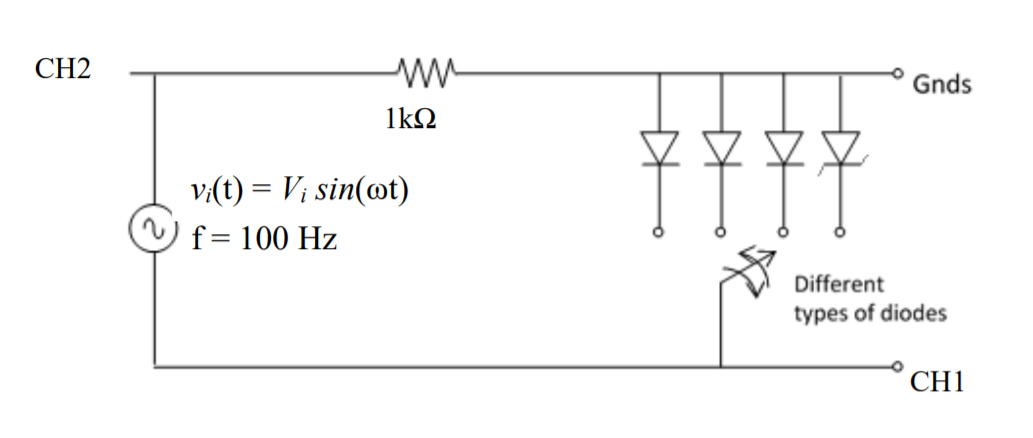
\includegraphics[width=1\textwidth]{1_1.png}
\caption{Circuit schematic for the step 1}
\end{figure} 

\subsubsection{a)}
\subsubsection{b)}

\subsection{Step 2}

\begin{figure}[H]
    \centering
    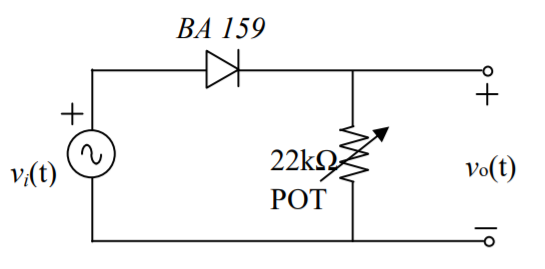
\includegraphics[width=1\textwidth]{2_1.png}
    \caption{Circuit schematic for the step 2}
\end{figure} 
    
\subsubsection{a)}
\subsubsection{b)}


\subsection{Step 3}

\begin{figure}[H]
    \centering
    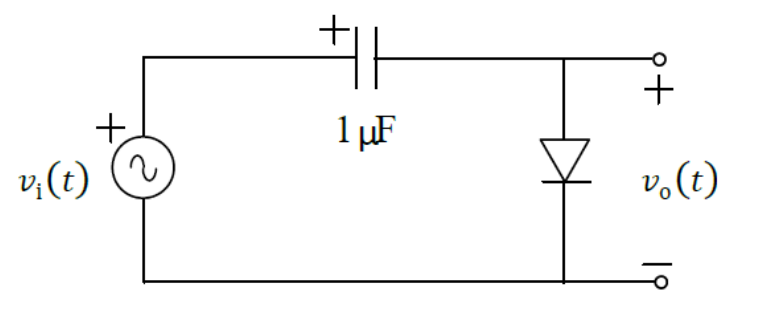
\includegraphics[width=1\textwidth]{3_1.png}
    \caption{Circuit schematic for the step 3}
\end{figure} 
    
    

\subsection{Step 4}

\begin{figure}[H]
    \centering
    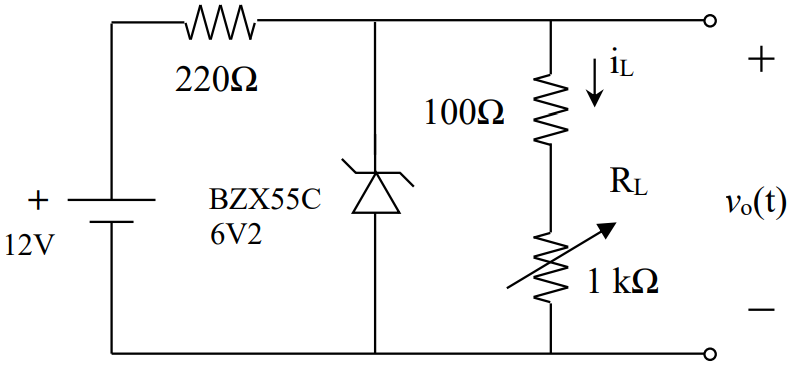
\includegraphics[width=1\textwidth]{4_1.png}
    \caption{Circuit schematic for the step 4}
\end{figure} 
    
    
\section{Conclusion}
asdfd
\section*{Appendix A}
\begin{itemize}
    \item PreLab Preprataion 6 hours
    \item Experimental Work 2  hours
    \item Report Wrining 6 hours
\end{itemize}

\end{document}

%%%%%%%%%%%%%%%%%%%%%%   EXAMPLE TABLE   %%%%%%%%%%%%%%%%%%%%%%%%%%%%%%%%
\begin{table}[H]
\begin{center}
    \caption{Resistance reading by color code convention.}
    \vspace{2mm}
    \begin{tabular}{||c | c | c||} 
        \hline
        Color Order & Value & Tolerance \\ [0.5ex] 
        \hline\hline
        Brown / Black / Red / Gold & 1k\( \Omega \) & \( \% \) 5  \\ 
        \hline
        Yellow / Violet / Red / Gold & 4.7k\( \Omega \) & \( \% \) 5   \\
        \hline
        Brown / Grey / Orange / Gold & 18k\( \Omega \) & \( \% \) 5  \\ [1ex] 
        \hline
    \end{tabular}
\end{center}
\end{table}


%%%%%%%%%%%%%%%%%%%%%%   EXAMPLE IMAGE   %%%%%%%%%%%%%%%%%%%%%%%%%%%%%%%%
\begin{figure}[H]
\centering
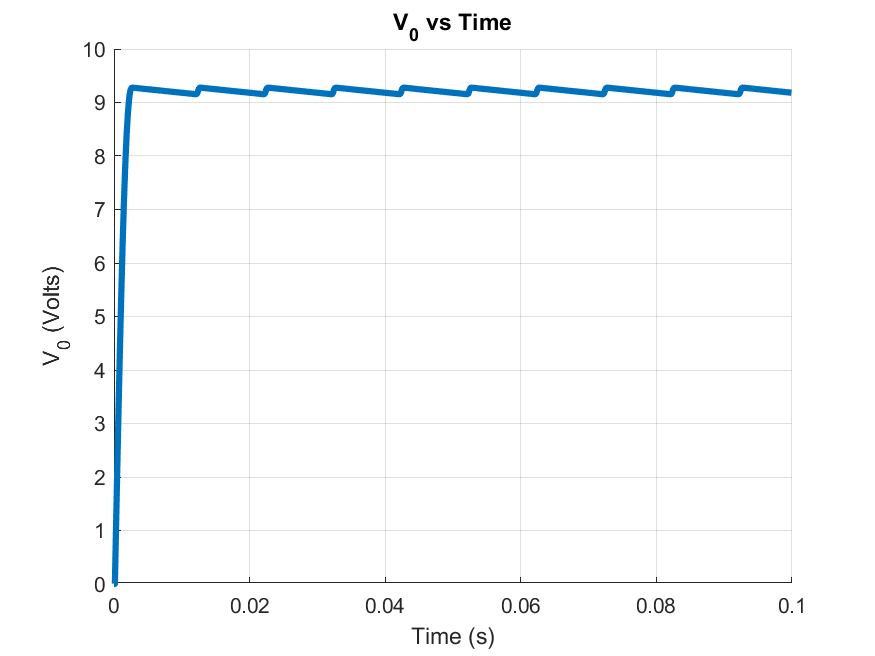
\includegraphics[width=1\textwidth]{5.png}
\caption{Circuit schematic for the step 5}
\end{figure} 

%%%%%%%%%%%%%%%%%%%%%%   EXAMPLE IMAGE FROM PDF   %%%%%%%%%%%%%%%%%%%%%%%%%%%%%%%%
\begin{figure}[H] \centering{
	\includegraphics[scale=0.25]{2a_plot.pdf}}
	\caption{Experiment 2}
\end{figure}
	